% !TEX program = pdflatex
% FRE6883 Recitation 1 -- Deck 4 -- C++ Syntax Practice
\documentclass[10pt,aspectratio=169]{beamer}

% Language & encoding
\usepackage[utf8]{inputenc}
\usepackage[T1]{fontenc}
\usepackage[english]{babel}
\usepackage{lmodern}
\usepackage{microtype}
\DisableLigatures{encoding=*,family=tt*}

% Math / tables / layout
\usepackage{amsmath,amssymb,bm,mathtools}
\usepackage{booktabs}
\usepackage{multicol}
\usepackage{changepage}

% Graphics
\usepackage{graphicx}
\usepackage{tikz}
\usetikzlibrary{arrows.meta,positioning,calc,decorations.pathreplacing}
\usepackage{pgfplots}
\pgfplotsset{compat=1.18}

% Theme (Metropolis)
\usetheme[numbering=fraction,progressbar=frametitle]{metropolis}
\setbeamertemplate{frame numbering}[fraction]
\setbeamertemplate{navigation symbols}{}

% Bootcamp palette
\definecolor{BootcampBlueDark}{HTML}{1A3C68}
\definecolor{BootcampBlue}{RGB}{31,110,178}
\definecolor{AccentGold}{HTML}{DAA520}
\definecolor{SoftGray}{RGB}{245,246,248}
\definecolor{TextBlack}{HTML}{000000}
\definecolor{Crimson}{HTML}{990000}
\definecolor{MatrixGreen}{HTML}{228B22}
\definecolor{MatrixRed}{HTML}{B22222}

% Global formatting
\setbeamercolor{normal text}{fg=TextBlack,bg=white}
\setbeamercolor{title}{fg=TextBlack}
\setbeamercolor{structure}{fg=BootcampBlueDark}
\setbeamercolor{progress bar}{fg=BootcampBlueDark,bg=gray!30}

\setbeamercolor{frametitle}{bg=BootcampBlueDark,fg=white}
\setbeamerfont{frametitle}{series=\bfseries,size=\large}
\setbeamertemplate{frametitle}{
  \nointerlineskip
  \begin{beamercolorbox}[wd=\paperwidth,ht=3.2ex,dp=1.4ex,leftskip=1em,rightskip=1em]{frametitle}
    \usebeamerfont{frametitle}\insertframetitle
  \end{beamercolorbox}
}

\setbeamercolor{block title example}{bg=BootcampBlueDark!90!black,fg=white}
\setbeamercolor{block body example}{bg=BootcampBlueDark!5!white,fg=black}
\setbeamercolor{block title proposition}{bg=MatrixGreen!75!black,fg=white}
\setbeamercolor{block body proposition}{bg=MatrixGreen!7!white,fg=black}
\setbeamercolor{block title illustration}{bg=AccentGold!85!black,fg=white}
\setbeamercolor{block body illustration}{bg=AccentGold!10!white,fg=black}
\setbeamercolor{block title proof}{bg=gray!70!black,fg=white}
\setbeamercolor{block body proof}{bg=SoftGray,fg=black}
\setbeamertemplate{blocks}[rounded][shadow=false]

\newenvironment{definitionblock}[1]{%
  \par\vspace{0.4em}%
  \begin{beamercolorbox}[
      wd=\textwidth,sep=0.4em,leftskip=0.3em,rightskip=0.6em,
      rounded=false,shadow=false
    ]{block title example}%
    \raisebox{0.15em}{\usebeamerfont{block title example}#1}%
  \end{beamercolorbox}%
  \vspace{-0.4em}%
  \begin{beamercolorbox}[
      wd=\textwidth,sep=0.9em,leftskip=0.6em,rightskip=0.6em,
      rounded=false,shadow=false
    ]{block body example}%
    \usebeamerfont{block body example}%
}{%
  \end{beamercolorbox}%
  \par\vspace{0.6em}%
}

\newenvironment{propositionblock}[1]{%
  \par\vspace{0.35em}%
  \begin{beamercolorbox}[
      wd=\textwidth,sep=0.4em,leftskip=0.3em,rightskip=0.6em,
      rounded=false,shadow=false
    ]{block title proposition}%
    \raisebox{0.15em}{\usebeamerfont{block title example}#1}%
  \end{beamercolorbox}%
  \vspace{-0.4em}%
  \begin{beamercolorbox}[
      wd=\textwidth,sep=0.8em,leftskip=0.6em,rightskip=0.6em,
      rounded=false,shadow=false
    ]{block body proposition}%
    \usebeamerfont{block body example}%
}{%
  \end{beamercolorbox}%
  \par\vspace{0.55em}%
}

\newenvironment{illustrationblock}[1]{%
  \par\vspace{0.35em}%
  \begin{beamercolorbox}[
      wd=\textwidth,sep=0.4em,leftskip=0.3em,rightskip=0.6em,
      rounded=false,shadow=false
    ]{block title illustration}%
    \raisebox{0.15em}{\usebeamerfont{block title example}#1}%
  \end{beamercolorbox}%
  \vspace{-0.4em}%
  \begin{beamercolorbox}[
      wd=\textwidth,sep=0.8em,leftskip=0.6em,rightskip=0.6em,
      rounded=false,shadow=false
    ]{block body illustration}%
    \usebeamerfont{block body example}%
}{%
  \end{beamercolorbox}%
  \par\vspace{0.55em}%
}

\newenvironment{proofblock}[1]{%
  \par\vspace{0.3em}%
  \begin{beamercolorbox}[
      wd=\textwidth,sep=0.35em,leftskip=0.3em,rightskip=0.6em,
      rounded=false,shadow=false
    ]{block title proof}%
    \raisebox{0.15em}{\usebeamerfont{block title example}#1}%
  \end{beamercolorbox}%
  \vspace{-0.4em}%
  \begin{beamercolorbox}[
      wd=\textwidth,sep=0.7em,leftskip=0.6em,rightskip=0.6em,
      rounded=false,shadow=false
    ]{block body proof}%
    \usebeamerfont{block body example}%
}{%
  \end{beamercolorbox}%
  \par\vspace{0.45em}%
}


\usepackage{listings}
\lstdefinestyle{coursecpp}{
  language=C++,
  basicstyle=\ttfamily\fontsize{10}{11.5}\selectfont,
  keywordstyle=\color{blue},
  commentstyle=\color{MatrixGreen},
  stringstyle=\color{Crimson},
  showstringspaces=false,
  columns=fullflexible,
  keepspaces=true,
  tabsize=4,
  breaklines=false,
  frame=none,
  aboveskip=0.5em,
  belowskip=0.5em
}
\lstset{style=coursecpp}
\setbeamercovered{invisible}




% Teaching blocks and coursecpp are copied from Deck 2 above.
% Listings preserve the course font, syntax colors, and brace conventions.
\usepackage{textcomp}
\lstdefinestyle{exercisecpp}{
  style=coursecpp,
  basicstyle=\ttfamily\fontsize{10}{11.5}\selectfont,
  aboveskip=0.1em,
  belowskip=0.1em,
  upquote=true
}
\lstset{style=exercisecpp}
\setlength{\parskip}{0.1em}
\newcommand{\exerciseinfo}[2]{%
  \textbf{#1}\hfill{\small #2}\par
}
\newcommand{\solutioninfo}[1]{%
  {\color{MatrixGreen!75!black}\textbf{#1 -- Solution}}\par
}
\newcommand{\context}[1]{{\small #1\par}}
\title{C++ Syntax Practice}
\author{}
\date{}
% Self-contained source. Build: latexmk -pdf Deck_4_Cpp_Syntax_Practice.tex
% Course source: Topic 2, pp. 4--5, 7--19, 21--32, 34--37.
% All 12 requested exercises are present, followed by one optional challenge.
% Each exercise has exactly one question frame, immediately followed by its
% solution frame. No overlays. Total: 28 frames (title + vector primer + 26).
% DEFAULT 55-MINUTE ROUTE: 1,3,4,6,7,8,9,10 (A/B),12.
% Budget 5 minutes work + 1 minute explanation per core exercise, plus 1 minute
% opening. Exercises 2,5,11 are optional reserves for this route. They remain
% in numerical order so the whole deck can also be taught consecutively.
% FULL ROUTE: about 74 minutes including all 12 and the 1-minute vector primer.
% Optional challenge: about 6 extra minutes. Optional 10C can replace A/B review.
% Basic: 1--6. Intermediate: 7--12. Challenge: 13.
% The vector primer precedes Exercise 10; only part C uses this optional type.
% Exercises 2,6,11 deliberately contain mistakes. Do not execute Exercise 6
% before repairing its indexing. Exercise 11 is an expected compilation error.
% Assume finite model inputs and successful numeric input throughout.
% Exercise 4 checks only S0>0 and U>D>0, not the full financial model.
% Exercise 12 uses a fixed-size array, valid terminal data, and a signed n.
% No variable-length arrays, pointer lesson, or container implementation.

\begin{document}

\begin{frame}[plain]
\relax
\vfill
{\usebeamerfont{title}C++ Syntax Practice\par}
\medskip
{\color{BootcampBlueDark}\rule{0.95\textwidth}{0.8pt}}
\bigskip
{\Large FRE6883 -- Financial Computation\par}
{\large Recitation 1 -- Deck 4\par}
\bigskip
\textbf{One exercise at a time.}\par

\end{frame}

% EXERCISE 1 -- Basic / core. Work 5 min; solution 1 min.
\begin{frame}[fragile]{Exercise 1: predict the output}
\relax
\exerciseinfo{Basic}{Core}
\context{Inside main(); \#include <iostream> is assumed.}
\begin{center}
\begin{minipage}{0.78\textwidth}
\begin{lstlisting}
int x = 5;
double y = x / 2;

std::cout << y << std::endl;
\end{lstlisting}
\end{minipage}
\end{center}
\begin{enumerate}
\item What is printed, and why?
\item What type does the expression \texttt{x / 2} have?
\item Change one literal so that the program prints \texttt{2.5}.
\end{enumerate}
\end{frame}

\begin{frame}[fragile]{Solution 1: the division happens first}
\relax
\solutioninfo{Basic}
\begin{columns}[T,onlytextwidth]
\begin{column}{0.47\textwidth}
\begin{lstlisting}
int x = 5;
double y = x / 2;
std::cout << y << std::endl;
\end{lstlisting}
\begin{definitionblock}{Original output}
{\Large\texttt{2}}
\end{definitionblock}
\end{column}
\begin{column}{0.49\textwidth}
\begin{lstlisting}
int x = 5;
double y = x / 2.0;
std::cout << y << std::endl;
\end{lstlisting}
\begin{propositionblock}{With a double operand}
{\Large\texttt{2.5}}
\end{propositionblock}
\end{column}
\end{columns}
\textbf{Both operands are int in \texttt{x / 2}.} Integer division produces
\texttt{2}; assigning that result to a \texttt{double} gives \texttt{2.0}.\par
\smallskip
Using \texttt{2.0} makes the division floating point. Default \texttt{cout}
formatting prints \texttt{2.0} as \texttt{2}.
\end{frame}

% EXERCISE 2 -- Basic / reserve in the 55-minute route.
\begin{frame}[fragile]{Exercise 2: find the type problem}
\relax
\exerciseinfo{Basic}{Optional reserve}
\context{Inside main(); \#include <iostream> is assumed.}
\begin{center}
\begin{minipage}{0.78\textwidth}
\begin{lstlisting}
int stockPrice = 106.75;
double rate = 3 / 100;

std::cout << stockPrice << " " << rate;
\end{lstlisting}
\end{minipage}
\end{center}
\begin{enumerate}
\item Is this valid C++? What value is stored in each variable?
\item Repair both initializations to preserve the intended values.
\item Which type suits a stock price, and which suits a count of steps?
\end{enumerate}
\end{frame}

\begin{frame}[fragile]{Solution 2: choose the type and the expression}
\relax
\solutioninfo{Basic}
\begin{center}
\begin{minipage}{0.78\textwidth}
\begin{lstlisting}
double stockPrice = 106.75;
double rate = 3.0 / 100.0;
int steps = 5;
\end{lstlisting}
\end{minipage}
\end{center}
\begin{propositionblock}{Original output: \texttt{106 0}}
\texttt{int stockPrice = 106.75;} is valid, but may produce a compiler warning.
Conversion to \texttt{int} discards the fractional part.\par
\smallskip
\texttt{3 / 100} is integer division, so \texttt{rate} receives \texttt{0.0}.
\end{propositionblock}
\textbf{Use \texttt{double} for decimal quantities and \texttt{int} for counts.}\par
The corrected rate is \texttt{0.03}; changing only its destination type cannot fix the division.
\end{frame}

% EXERCISE 3 -- Basic / core. Numeric input is assumed valid.
\begin{frame}[fragile]{Exercise 3: complete the call payoff}
\relax
\exerciseinfo{Basic}{Core}
\context{Inside main(); \#include <iostream> is assumed. The user enters a number.}
\begin{columns}[T,onlytextwidth]
\begin{column}{0.55\textwidth}
\begin{lstlisting}
double S = 0.0, K = 100.0;
std::cin >> S;
double payoff = 0.0;
if (S > K)
{
    // complete this line
}
else
{
    // complete this line
}
std::cout << payoff;
\end{lstlisting}
\end{column}
\begin{column}{0.41\textwidth}
\begin{enumerate}
\item Complete the European call payoff.
\item What is printed for inputs \texttt{90}, \texttt{100}, and \texttt{106}?
\item Which path is taken when \texttt{S == K}?
\end{enumerate}
\end{column}
\end{columns}
\end{frame}

\begin{frame}[fragile]{Solution 3: one condition, two paths}
\relax
\solutioninfo{Basic}
\begin{columns}[T,onlytextwidth]
\begin{column}{0.51\textwidth}
\begin{lstlisting}
if (S > K)
{
    payoff = S - K;
}
else
{
    payoff = 0.0;
}
std::cout << payoff;
\end{lstlisting}
\end{column}
\begin{column}{0.45\textwidth}
\begin{propositionblock}{Check the boundary}
\begin{tabular}{@{}rr@{}}
\textbf{Input S} & \textbf{Output} \\
90 & 0 \\
100 & 0 \\
106 & 6
\end{tabular}
\end{propositionblock}
\texttt{S > K} is a comparison. Only one path executes.\par
\smallskip
At equality, the condition is false, so \texttt{else} assigns zero.
\end{column}
\end{columns}
\smallskip
\texttt{std::cin >> S} reads input;
\texttt{payoff = S - K} assigns the computed value.
\end{frame}

% EXERCISE 4 -- Basic / core. Simplified validity, not an arbitrage test.
\begin{frame}[fragile]{Exercise 4: complete the validation}
\relax
\exerciseinfo{Basic}{Core}
\context{Inside main(); S0, U, D are finite doubles. Assume \#include <iostream>.}
\begin{lstlisting}
if (S0 <= 0.0 ___ U <= D ___ D <= 0.0)
{
    std::cout << "Invalid parameters";
}
\end{lstlisting}
\begin{enumerate}
\item Fill the blanks to validate $S_0>0$ and $U>D>0$.
\item Which inputs below are rejected? Explain each decision.
\item Write one condition that is true exactly when these inputs are valid.
\end{enumerate}
\smallskip
\centering
\begin{tabular}{@{}lrrr@{}}
\toprule
\textbf{Case} & \textbf{S0} & \textbf{U} & \textbf{D} \\
\midrule
A & 100.0 & 1.2 & 0.8 \\
B & 100.0 & 0.9 & 1.1 \\
C & 0.0 & 1.2 & 0.8 \\
\bottomrule
\end{tabular}
\end{frame}

\begin{frame}[fragile]{Solution 4: reject any invalid component}
\relax
\solutioninfo{Basic}
\begin{lstlisting}
if (S0 <= 0.0 || U <= D || D <= 0.0)
{
    std::cout << "Invalid parameters";
}
\end{lstlisting}
\begin{propositionblock}{\texttt{||} means OR; \texttt{\&\&} means AND}
An OR condition is true when at least one component is true.\par
The valid-input condition requires \textbf{all} three checks:
\begin{lstlisting}
S0 > 0.0 && U > D && D > 0.0
\end{lstlisting}
\end{propositionblock}
\textbf{A passes. B fails because \texttt{U <= D}. C fails because \texttt{S0 <= 0.0}.}\par
\smallskip
{\small These are the simplified checks $S_0>0$ and $U>D>0$; the full model also checks R.}
\end{frame}

% EXERCISE 5 -- Basic / reserve in the 55-minute route.
\begin{frame}[fragile]{Exercise 5: trace a for loop}
\relax
\exerciseinfo{Basic}{Optional reserve}
\context{Inside main(); \#include <iostream> is assumed.}
\begin{center}
\begin{minipage}{0.78\textwidth}
\begin{lstlisting}
for (int i = 0; i < 5; i++)
{
    std::cout << i << " ";
}
\end{lstlisting}
\end{minipage}
\end{center}
\begin{enumerate}
\item What is printed? How many times does the body execute?
\item What changes if the condition becomes \texttt{i <= 5}?
\item Rewrite the loop to print the integers from 4 down to 0.
\end{enumerate}
\end{frame}

\begin{frame}[fragile]{Solution 5: initialize, test, execute, update}
\relax
\solutioninfo{Basic}
\begin{columns}[T,onlytextwidth]
\begin{column}{0.47\textwidth}
\begin{definitionblock}{Original loop}
\texttt{0 1 2 3 4}\par
\textbf{5 iterations.} At \texttt{i == 5}, the test fails.
\end{definitionblock}
\begin{propositionblock}{With \texttt{i <= 5}}
\texttt{0 1 2 3 4 5}\par
\textbf{6 iterations.} Equality is included.
\end{propositionblock}
\end{column}
\begin{column}{0.49\textwidth}
\begin{lstlisting}
for (int i = 4; i >= 0; i--)
{
    std::cout << i << " ";
}
\end{lstlisting}
\texttt{4 3 2 1 0}\par
\smallskip
\texttt{i++} adds one; \texttt{i--} subtracts one.
\end{column}
\end{columns}
\textbf{A for loop tests its condition before each execution of the body.}\par
{\small Each example also prints one space after its final number.}
\end{frame}

% EXERCISE 6 -- Basic / core. Diagnose only; never run the invalid write.
\begin{frame}[fragile]{Exercise 6: find the indexing bug}
\relax
\exerciseinfo{Basic}{Core}
\context{Inside main(). Diagnose this code on paper before running it.}
\begin{center}
\begin{minipage}{0.78\textwidth}
\begin{lstlisting}
double prices[5];

for (int i = 0; i <= 5; i++)
{
    prices[i] = 100.0;
}
\end{lstlisting}
\end{minipage}
\end{center}
\begin{enumerate}
\item What is wrong, and at which iteration does it happen?
\item Which indices belong to this array?
\item Correct the loop so that every element is assigned exactly once.
\end{enumerate}
\end{frame}

\begin{frame}[fragile]{Solution 6: the last index is size minus one}
\relax
\solutioninfo{Basic}
\begin{columns}[T,onlytextwidth]
\begin{column}{0.50\textwidth}
\begin{lstlisting}
double prices[5];

for (int i = 0; i < 5; i++)
{
    prices[i] = 100.0;
}
\end{lstlisting}
\end{column}
\begin{column}{0.46\textwidth}
\begin{propositionblock}{Valid indices: 0, 1, 2, 3, 4}
\textbf{Use \texttt{i < 5}.}\par
The original sixth iteration writes to \texttt{prices[5]}, outside the array.
\end{propositionblock}
\end{column}
\end{columns}
Raw C++ arrays provide \textbf{no automatic bounds checking}.
An invalid access has undefined behavior; a crash is not guaranteed.\par
\smallskip
The corrected loop assigns every element before it is read.
\end{frame}

% EXERCISE 7 -- Intermediate / core.
\begin{frame}[fragile]{Exercise 7: visit the tree nodes}
\relax
\exerciseinfo{Intermediate}{Core}
\context{Inside main(); \#include <iostream> is assumed.}
\begin{columns}[T,onlytextwidth]
\begin{column}{0.60\textwidth}
\begin{lstlisting}
const int N = 3;
for (int n = 0; n <= N; n++)
{
    for (int i = 0; i <= n; i++)
    {
        std::cout << "(" << n << ","
                  << i << ") ";
    }
}
\end{lstlisting}
\end{column}
\begin{column}{0.36\textwidth}
\begin{enumerate}
\item How many times is the inner body executed in total?
\item List the pairs \texttt{(n,i)} in execution order.
\item Why is this loop structure natural for a binomial tree?
\end{enumerate}
\end{column}
\end{columns}
\end{frame}

\begin{frame}{Solution 7: the inner loop restarts on each row}
\relax
\solutioninfo{Intermediate}
\begin{center}
\renewcommand{\arraystretch}{1.15}
\begin{tabular}{@{}clc@{}}
\toprule
\textbf{n} & \textbf{Pairs visited, in order} & \textbf{Executions} \\
\midrule
0 & \texttt{(0,0)} & 1 \\
1 & \texttt{(1,0), (1,1)} & 2 \\
2 & \texttt{(2,0), (2,1), (2,2)} & 3 \\
3 & \texttt{(3,0), (3,1), (3,2), (3,3)} & 4 \\
\bottomrule
\end{tabular}
\end{center}
\begin{propositionblock}{Total: $1+2+3+4=10$ executions}
At time step \texttt{n}, the tree has \texttt{n + 1} nodes, indexed from 0 through n.
The inner loop initializes \texttt{i = 0} again for each new n.
\end{propositionblock}
\textbf{n selects the time step; i selects a node within that time step.}
\end{frame}

% EXERCISE 8 -- Intermediate / core. Function and file organization together.
\begin{frame}[fragile]{Exercise 8: complete and organize a function}
\relax
\exerciseinfo{Intermediate}{Core}
\context{Use the course relation $S(n,i)=S_0 U^i D^{n-i}$; assume $0\leq i\leq n$.}
\begin{lstlisting}
double CalculateAssetPrice(double S0, double U,
                           double D, int n, int i)
{
    // complete
}
\end{lstlisting}
\begin{enumerate}
\item Complete the function body.
\item Identify the return type and the type of each parameter.
\item Write its declaration in \texttt{BinomialTreeModel.h}, inside namespace \texttt{fre}.
\item Where does the definition belong, and how does \texttt{main()} call it?
\end{enumerate}
\end{frame}

\begin{frame}[fragile]{Solution 8: a declaration promises; a definition implements}
\relax
\solutioninfo{Intermediate}
\begin{columns}[T,onlytextwidth]
\begin{column}{0.46\textwidth}
\textbf{BinomialTreeModel.h}
\begin{lstlisting}[basicstyle=\ttfamily\fontsize{9.5}{10.5}\selectfont]
#pragma once
namespace fre
{
double CalculateAssetPrice(
    double S0, double U, double D,
    int n, int i);
}
\end{lstlisting}
{\small\textbf{Main.cpp:} include the header, then call:}
\begin{lstlisting}[basicstyle=\ttfamily\fontsize{9.5}{10.5}\selectfont]
fre::CalculateAssetPrice(
    100.0, 1.2, 0.8, 2, 1);
\end{lstlisting}
{\small\textbf{double:} result, S0, U, D.\par
\textbf{int:} n, i. \quad \textbf{fre::} selects the namespace.}
\end{column}
\begin{column}{0.50\textwidth}
\textbf{BinomialTreeModel.cpp}
\begin{lstlisting}[basicstyle=\ttfamily\fontsize{9.5}{10.5}\selectfont]
#include "BinomialTreeModel.h"
#include <cmath>
namespace fre
{
double CalculateAssetPrice(
    double S0, double U, double D,
    int n, int i)
{
    return S0 * std::pow(U, i)
           * std::pow(D, n - i);
}
}
\end{lstlisting}
\end{column}
\end{columns}
\smallskip
{\small The header declares; the function body defines. Compile both \texttt{.cpp} files together.}
\end{frame}

% EXERCISE 9 -- Intermediate / core.
\begin{frame}[fragile]{Exercise 9: trace a function call}
\relax
\exerciseinfo{Intermediate}{Core}
\context{Complete program; \#include <iostream> is assumed.}
\begin{columns}[T,onlytextwidth]
\begin{column}{0.51\textwidth}
\begin{lstlisting}
void Foo(int a, int& b)
{
    a++;
    b++;
}
int main()
{
    int x = 1;
    int y = 1;
    Foo(x, y);
    std::cout << x << " " << y;
}
\end{lstlisting}
\end{column}
\begin{column}{0.45\textwidth}
\begin{enumerate}
\item What is printed after \texttt{Foo(x, y)}?
\item Track \texttt{a}, \texttt{b}, \texttt{x}, and \texttt{y} through the call.
\item What changes if the first parameter becomes \texttt{int\& a}?
\end{enumerate}
\end{column}
\end{columns}
\end{frame}

\begin{frame}{Solution 9: a copy and an alias behave differently}
\relax
\solutioninfo{Intermediate}
\begin{propositionblock}{Output: \texttt{1 2}}
\texttt{int a} receives a \textbf{copy} of x. Incrementing a changes only that copy.\par
\smallskip
\texttt{int\& b} is an \textbf{alias} for y. Incrementing b changes y itself.
\end{propositionblock}
\begin{center}
\renewcommand{\arraystretch}{1.25}
\begin{tabular}{@{}lcc@{}}
\toprule
 & \textbf{On entry to Foo} & \textbf{After both increments} \\
\midrule
\texttt{x} in main & 1 & 1 \\
\texttt{a}, the copy & 1 & 2 \\
\texttt{y}, also named b & 1 & 2 \\
\bottomrule
\end{tabular}
\end{center}
\textbf{With \texttt{int\& a}, both arguments are modified: the output becomes \texttt{2 2}.}
\end{frame}

% Optional primer -- 1 minute only if using Exercise 10C.
\begin{frame}[fragile]{Optional extension: reading a vector type}
\relax
\exerciseinfo{Intermediate}{Before Exercise 10C only}
\begin{definitionblock}{One new type name}
\texttt{std::vector<double>} denotes a sequence of doubles.
Its type comes from \texttt{<vector>}; \texttt{std::} is the standard-library namespace.
\end{definitionblock}
\begin{center}
\begin{minipage}{0.78\textwidth}
\begin{lstlisting}
#include <vector>

// Inside main():
std::vector<double> prices = {100.0, 102.0, 98.0};
\end{lstlisting}
\end{minipage}
\end{center}
\texttt{prices[0]}, \texttt{prices[1]}, and \texttt{prices[2]} name the three elements.\par
\smallskip
{\small Exercise 10C only asks you to choose a parameter type.
No vector implementation is required. Skip this extension if the type is new to the group.}
\end{frame}

% EXERCISE 10 -- Intermediate / core A/B; optional extension C.
\begin{frame}[fragile]{Exercise 10: choose the parameter type}
\relax
\exerciseinfo{Intermediate}{Core A/B; optional C}
\begin{columns}[T,onlytextwidth]
\begin{column}{0.51\textwidth}
\begin{lstlisting}
// A: square x; keep caller unchanged.
double Square( ??? x );

// B: read into the caller's variable.
void ReadPrice( ??? price );

// C (optional): mean of a big vector.
// Read only; assume it is nonempty.
double Mean( ??? prices );
\end{lstlisting}
\end{column}
\begin{column}{0.45\textwidth}
\textbf{Choose from:}\par
\texttt{double}\par
\texttt{double\&}\par
\texttt{const double\&}\par
\texttt{std::vector<double>}\par
\texttt{std::vector<double>\&}\par
\texttt{const std::vector<double>\&}
\end{column}
\end{columns}
\begin{enumerate}
\item Choose a suitable type for each parameter and explain why.
\item Write the one-line bodies of A and B, assuming valid numeric input.
\item Would another type compile but be less suitable for the stated task?
\end{enumerate}
\end{frame}

\begin{frame}[fragile]{Solution 10: match the parameter to its job}
\relax
\solutioninfo{Intermediate}
\begin{columns}[T,onlytextwidth]
\begin{column}{0.47\textwidth}
\begin{lstlisting}
double Square(double x)
{
    return x * x;
}

void ReadPrice(double& price)
{
    std::cin >> price;
}
\end{lstlisting}
\end{column}
\begin{column}{0.49\textwidth}
\textbf{A: pass a small read-only value by value.}\par
Copying one \texttt{double} is inexpensive.\par
\smallskip
\textbf{B: use a reference to modify the caller.}\par
A value parameter would only update a copy.\par
\smallskip
\textbf{C: use a const reference for a large read-only object.}\par
Avoid copying the vector; forbid edits through this parameter.
\end{column}
\end{columns}
\begin{lstlisting}
double Mean(const std::vector<double>& prices); // optional C
\end{lstlisting}
{\small \texttt{const double\&} also works for A but is unnecessary here.
C by value copies the vector; a non-const reference permits edits through the parameter.}
\end{frame}

% EXERCISE 11 -- Intermediate / reserve in the 55-minute route.
\begin{frame}[fragile]{Exercise 11: does this function compile?}
\relax
\exerciseinfo{Intermediate}{Optional reserve}
\begin{center}
\begin{minipage}{0.78\textwidth}
\begin{lstlisting}
void Foo(const int& x)
{
    x++;
}
\end{lstlisting}
\end{minipage}
\end{center}
\begin{enumerate}
\item Does this compile? Explain the rule involved.
\item What does \texttt{const} guarantee through this parameter?
\item Change the parameter type to modify the caller; then give a type that modifies only a copy.
\end{enumerate}
\end{frame}

\begin{frame}[fragile]{Solution 11: const prevents writes through x}
\relax
\solutioninfo{Intermediate}
\begin{propositionblock}{The original function does not compile}
\texttt{x++} attempts to modify an object through \texttt{const int\& x}.
The reference allows reading, but not modifying, that object through x.
\end{propositionblock}
\begin{columns}[T,onlytextwidth]
\begin{column}{0.47\textwidth}
\textbf{Modify the caller}
\begin{lstlisting}
void Foo(int& x)
{
    x++;
}
\end{lstlisting}
\end{column}
\begin{column}{0.49\textwidth}
\textbf{Modify only a local copy}
\begin{lstlisting}
void Foo(int x)
{
    x++;
}
\end{lstlisting}
\end{column}
\end{columns}
{\small A const reference does not make the caller's variable permanently const.
The caller can still modify its own non-const variable.}
\end{frame}

% EXERCISE 12 -- Intermediate / core. Conceptual reading, no price derivation.
\begin{frame}[fragile]{Exercise 12: read the backward loop}
\relax
\exerciseinfo{Intermediate}{Core}
\context{N = 3; Price has 4 elements holding terminal option payoffs. R > 0; 0 < q < 1.}
\begin{columns}[T,onlytextwidth]
\begin{column}{0.55\textwidth}
\begin{lstlisting}
for (int n = N - 1; n >= 0; n--)
{
    for (int i = 0; i <= n; i++)
    {
        Price[i] =
            (q * Price[i + 1]
            + (1.0 - q) * Price[i]) / R;
    }
}
\end{lstlisting}
\end{column}
\begin{column}{0.41\textwidth}
\begin{enumerate}
\item Why does n decrease, and which values does it take?
\item Why stop the inner loop at \texttt{i <= n}?
\item What does \texttt{Price[i]} represent just before and just after its assignment?
\item Which next-step values are used, and why is this backward induction?
\end{enumerate}
\end{column}
\end{columns}
\end{frame}

\begin{frame}{Solution 12: replace the next row with the current row}
\relax
\solutioninfo{Intermediate}
\begin{center}
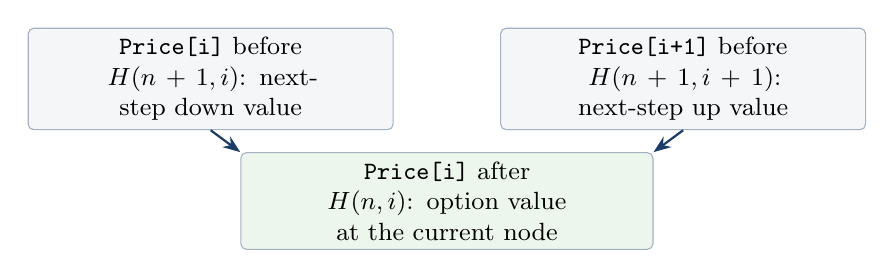
\begin{tikzpicture}[
  box/.style={draw=BootcampBlueDark!40,fill=SoftGray,
    rounded corners=2pt,align=center,minimum height=1.1cm,
    text width=4.4cm,font=\small},
  flow/.style={-{Stealth[length=2.2mm]},thick,draw=BootcampBlueDark}
]
\node[box] (down) at (-3.0,1.55) {\texttt{Price[i]} before\\$H(n+1,i)$: next-step down value};
\node[box] (up) at (3.0,1.55) {\texttt{Price[i+1]} before\\$H(n+1,i+1)$: next-step up value};
\node[box,fill=MatrixGreen!8,text width=5.0cm] (now) at (0,0)
  {\texttt{Price[i]} after\\$H(n,i)$: option value at the current node};
\draw[flow] (down.south) -- (now.north west);
\draw[flow] (up.south) -- (now.north east);
\end{tikzpicture}
\end{center}
\textbf{For N = 3, n takes 2, 1, 0:} move from known terminal payoffs back toward today.\par
\smallskip
Row n has \textbf{n + 1 nodes}, indexed 0 through n.
At each assignment, \texttt{Price[i]} and \texttt{Price[i+1]} still hold next-step values.\par
\smallskip
{\small The forward inner loop reads both values before overwriting \texttt{Price[i]}.
After the final row, \texttt{Price[0]} holds today's option value.}
\end{frame}

% EXERCISE 13 -- Optional challenge. Work 5 min; solution 1 min.
\begin{frame}[fragile]{Exercise 13: find the largest price}
\relax
\exerciseinfo{Challenge}{Optional}
\context{Assume size > 0, the array contains at least size finite values, and no edits are allowed.}
\begin{center}
\begin{minipage}{0.87\textwidth}
\begin{lstlisting}
double MaxPrice(const double prices[], int size);
\end{lstlisting}
\end{minipage}
\end{center}
\begin{enumerate}
\item Write the function definition using a loop.
\item Test it on \texttt{\{100.0, 120.0, 90.0, 110.0\}}, then on \texttt{\{106.75\}}.
\item Explain the indices your loop visits and why your initialization works.
\end{enumerate}
\smallskip
{\small Use variables, comparisons, indexing, and a loop; no library maximum algorithm.}
\end{frame}

\begin{frame}[fragile]{Solution 13: carry the largest value seen so far}
\relax
\solutioninfo{Challenge}
\begin{columns}[T,onlytextwidth]
\begin{column}{0.60\textwidth}
\begin{lstlisting}
double MaxPrice(const double prices[],
                int size)
{
    double largest = prices[0];
    for (int i = 1; i < size; i++)
    {
        if (prices[i] > largest)
        {
            largest = prices[i];
        }
    }
    return largest;
}
\end{lstlisting}
\end{column}
\begin{column}{0.36\textwidth}
\begin{propositionblock}{Start from a real element}
\raggedright
\texttt{largest} is the maximum of all elements visited so far.
\end{propositionblock}
\textbf{Results:} \texttt{120.0} and \texttt{106.75}.\par
\smallskip
With one element, the loop runs zero times and returns \texttt{prices[0]}.
\smallskip\par
{\small Assume \texttt{size > 0}; \texttt{const} prevents edits through \texttt{prices}.}
\end{column}
\end{columns}
\end{frame}

\end{document}
